\section{Resoconto attività di verifica}
In questa sezione vengono descritti e analizzati gli esiti delle attività
di verifica svolte su tutti i documenti che vengono consegnati nelle varie 
revisioni di avanzamento del progetto.

\subsection{Revisione dei requisiti}

%\subsubsection{Analisi statica dei documenti}
%L'analisi dei documenti mediante \textit{Walkthrough}\glo{} ha portato 
%all'individuazione di alcuni errori frequenti a partire dai quali è stata 
%stilata una lista di controllo interna.

\subsubsection{Qualità di processo}

Di seguito vengono riportati gli esiti delle metriche derivanti dalla gestione di qualità di processi, seguiti dalla tabella degli indici di Gulpease e degli indici di Gunning Fog che riporta gli esiti di tutti i documenti prodotti finora. \\
\textbf{Leggenda}:
\begin{itemize}
	\item \textbf{N.C.} - Non Calcolabile;
	\item \textbf{S} - Superato;
	\item \textbf{N.S.} - Non Superato;
	\item \textbf{\%} - Percentuale;
	\item \textbf{V} - Valore numerico;
	\item \textbf{\euro{}} - Euro.
\end{itemize}
	\rowcolors{2}{pari}{dispari}	
	\begin{longtable}{ >{\centering}p{0.25\textwidth} >{\centering}p{0.10\textwidth}
			 >{\centering}p{0.10\textwidth} >{\centering}p{0.07\textwidth} >{\centering}p{0.31\textwidth}}
		\caption{ Valutazione della qualità di processo - RR} \\
		%\hline
		\rowcolorhead
		
		\centering\textbf{\color{white}Codice - nome metrica} 
		& \centering\textbf{\color{white}Unità di misura} 
		& \centering\textbf{\color{white}Valore} 
		& \centering\textbf{\color{white}Esito}
		& \centering\textbf{\color{white}Accettazione}
		\tabularnewline %\hline 
		\endfirsthead
		
		Requisiti obbligatori soddisfatti & \% & N.C. & N.S. & 100
		\tabularnewline 
		
		Coupling Between Object classes & V & N.C. & N.S. & $0 \leq CBO \leq 6$
		\tabularnewline
		
		Planned Value & \euro{} & 4.688,00 & S & $ \geq 0$
		\tabularnewline
		
		Actual Cost & \euro{} & 4.833,00 & S & $0 \leq AC \leq 11.689,00 $
		\tabularnewline
		
		Earned Value & \euro{} & 4.688,00 & S & $ \geq 0$
		\tabularnewline
		
		Budget at Completion & \euro{} & 4.688,00 & S & $4.591,35 \leq BAC \leq 5074,65 $
		\tabularnewline
		
		Cost Variance & \euro{} & -145,00 & N.S. & $ \geq 0$
		\tabularnewline
		
		Schedule Variance & \euro{} & 0,00 & S & $ \geq 0$
		\tabularnewline
		
		Code Coverage & \% & N.C. & N.S. & $75\%$
		\tabularnewline
		
		Indice Gunning fog (media) & V & 13,71 & S & $ \leq 16$
		\tabularnewline
		
		Indice di Gulpease (media) & V & 68,54 & S & $40 < I_G < 100$
		\tabularnewline
		
		Correttezza ortografica & V & 0 & S & 0
		\tabularnewline
		
		Percentuale di metriche soddisfatte & \% & 88,89 & S & 100
		\tabularnewline
		
	\end{longtable}
	
	\paragraph{Considerazioni}
	Ci sono delle metriche non calcolabili in questa fase. Queste ultime si riferiscono all'analisi del codice e alla sua progettazione di dettaglio che verrà svolta nelle fasi successive.
	Risulta invece negativa la metrica di Cost Variance, in conseguenza dell'impiego di 8 ore di lavoro aggiuntive rispetto a quanto previsto. \\
	La percentuale di metriche soddisfatte tiene conto solo delle metriche calcolabili, quindi di un totale di 9 tra cui 8 soddisfatte; se si ritiene che le metriche non calcolabili siano da considerare non superate, la percentuale di metriche soddisfatte risulta comunque superata, per un valore di 66.67.

	\rowcolors{2}{pari}{dispari}
	\begin{longtable}{ >{\centering}p{0.40\textwidth} >{\centering}p{0.25\textwidth}
			 >{\centering}p{0.2075\textwidth} }
		\caption{ Verifiche automatizzate indice di Gulpease - RR} \\
		%\hline
		\rowcolorhead
		\centering\textbf{\color{white}Documento} 
		& \centering\textbf{\color{white}Indice Gulpease} 
		& \centering\textbf{\color{white}Esito}
		\tabularnewline %\hline 
		\endfirsthead
			
	
		\textit{Analisi dei Requisiti v2.0.0} & 52,32 & Superato
		
		\tabularnewline 
		\textit{Glossario v2.0.0} & 100 & Superato
				
		\tabularnewline 
		\textit{Norme di Progetto v2.0.0} & 57,61 & Superato
		
		\tabularnewline 
		\textit{Piano di Progetto v2.0.0} & 53,39 & Superato
		
		\tabularnewline 
		\textit{Piano di Qualifica v2.0.0} & 56,87 & Superato	
		
		\tabularnewline 
		\textit{Studio di Fattibilità v1.0.0} & 54,93 & Superato
		
		\tabularnewline 
		\textit{Verbale Esterno 2019-03-14 v1.0.0} & 80 & Superato
		
		\tabularnewline 
		\textit{Verbale Esterno 2019-03-25 v1.0.0} & 72 & Superato
		
		\tabularnewline 
		\textit{Verbale Esterno 2019-04-10 v1.0.0} & 69 & Superato
		
		\tabularnewline 
		\textit{Verbale Interno 2019-03-06 v1.0.0} & 79 & Superato
		
		\tabularnewline 
		\textit{Verbale Interno 2019-03-13 v1.0.0} & 77 & Superato
		
		\tabularnewline 
		\textit{Verbale Interno 2019-03-18 v1.0.0} & 71 & Superato
	\end{longtable}
	\subparagraph*{Considerazioni} 
	Tutti i documenti hanno un esito positivo. La media dei valori è di 68.54, un valore intermedio tra il limite inferiore stabilito di 40 e il limite inferiore preferibile di 80. \\
	I valori più alti sono riscontrati nei verbali e glossario, mentre i valori più bassi sono presenti nell'\texttt{AdR} e nel \texttt{PdP} ma data la loro natura tecnica, riteniamo soddisfacente l'esito della verifica.
	
	
	
	\rowcolors{2}{pari}{dispari}
	\begin{longtable}{ >{\centering}p{0.40\textwidth} >{\centering}p{0.25\textwidth}
			 >{\centering}p{0.2075\textwidth}}
		\caption{ Verifiche automatizzate indice di Gunning Fog  - RR} \\
		%\hline
		\rowcolorhead
		\centering\textbf{\color{white}Documento} 
		& \centering\textbf{\color{white}Indice Gunning Fog} 
		& \centering\textbf{\color{white}Esito}
		\tabularnewline %\hline 
		\endfirsthead
			
		\textit{Analisi dei Requisiti v2.0.0} & 13,06 & Superato
		
		\tabularnewline 
		\textit{Glossario v2.0.0} & 12,32 & Superato
				
		\tabularnewline 
		\textit{Norme di Progetto v2.0.0} & 11,70  & Superato
		
		\tabularnewline 
		\textit{Piano di Progetto v2.0.0} & 12,29 & Superato
		
		\tabularnewline 
		\textit{Piano di Qualifica v2.0.0} & 12,71 & Superato	
		
		\tabularnewline 
		\textit{Studio di Fattibilità v1.0.0} & 11,28 & Superato
		
		\tabularnewline 
		\textit{Verbale Esterno 2019-03-14 v1.0.0} & 14,81 & Superato
		
		\tabularnewline 
		\textit{Verbale Esterno 2019-03-25 v1.0.0} & 15,59 & Superato
		
		\tabularnewline 
		\textit{Verbale Esterno 2019-04-10 v1.0.0} & 15,77  & Superato
		
		\tabularnewline 
		\textit{Verbale Interno 2019-03-06 v1.0.0} & 13,96 & Superato
		
		\tabularnewline 
		\textit{Verbale Interno 2019-03-13 v1.0.0} & 15,44 & Superato
		
		\tabularnewline 
		\textit{Verbale Interno 2019-03-18 v1.0.0} & 15,62 & Superato
	\end{longtable}
	\subparagraph*{Considerazioni} 
	Tutti i documenti hanno superato la verifica con un esito inferiore al limite massimo imposto di 16. 
	Con una media di 13.71, in cui i documenti più rilevanti hanno un esito vicino al valore preferibile di 12, riteniamo che la verifica abbia riportato dei risultati soddisfacenti. 
	
\subsubsection{Qualità di prodotto}
	
	\paragraph{Considerazioni}
	Data la non implementazione del prodotto software, nella fase attuale le metriche derivanti dalla gestione della qualità di prodotto non possono essere calcolate.
\subsubsection{Esito RR}
	In seguito alla valutazione della prima revisione, il gruppo ha apportato varie modifiche basandosi sulle segnalazioni ricevute. Di seguito vengono descritte brevemente tali modifiche:
	\begin{itemize}
		\item corrette le difformità nei titoli dei vari documenti;
		\item \textbf{Norme di progetto}: 
			\begin{itemize}	
				\item inserito lo standard ISO/IEC 12207 come riferimento informativo;
				\item modificato §2.1 del Processo di Fornitura, descrivendo le attività previste dallo standard ISO/IEC 12207 di interesse per il gruppo;
				\item aggiunto maggiore dettaglio a §2.2 del Processo di Sviluppo;
				\item aggiunto §4.2 che tratta il processo di Fornitura.
			\end{itemize}
		\item \textbf{Analisi dei Requisiti}: 
			\begin{itemize}
				\item corretti tutti i casi d'uso secondo le indicazioni ricevute;
				\item aggiunto UC24, UC25, UC26 e UC27 per completare il tracciamento requisiti - casi d'uso.
			\end{itemize} 
		\item \textbf{Piano di Progetto}: 
			\begin{itemize}
				\item modificata la pianificazione delle fasi successive all'RR, cercando di seguire il modello incrementale;
				\item modificato il titolo di §6 in "Consuntivo di periodo" e inserito paragrafo "Conclusioni" con relativa analisi e considerazioni del periodo a precedere.
			\end{itemize}
		\item \textbf{Piano di Qualifica}: 
			\begin{itemize}
				\item stabiliti obiettivi e strategie per garantire la qualità del processo di Fornitura, in seguito all'analisi dello standard ISO/IEC 12207:1995 §5.2;
				\item inserita tabella riportante gli esiti delle metriche calcolabile in fase RR.
			\end{itemize}
	\end{itemize}

	\paragraph{Considerazioni}
		In generale, risulta che i documenti abbiano un buona struttura ma che siano scarsi per contenuti. \\
		Il gruppo si è impegnato a integrare i contenuti ritenuti insoddisfacenti e ad aggiungere maggiore dettaglio nella loro descrizione.
		\newpage
		
\subsection{Revisione di progettazione}

\subsubsection{Qualità di processo}

Di seguito vengono riportati gli esiti delle metriche derivanti dalla gestione di qualità di processi, seguiti dalla tabella degli indici di Gulpease e degli indici di Gunning Fog che riporta gli esiti di tutti i documenti prodotti finora. \\
\textbf{Leggenda}:
\begin{itemize}
	\item \textbf{N.C.} - Non Calcolabile;
	\item \textbf{S} - Superato;
	\item \textbf{N.S.} - Non Superato;
	\item \textbf{\%} - Percentuale;
	\item \textbf{V} - Valore numerico;
	\item \textbf{\euro{}} - Euro.
\end{itemize}
	\rowcolors{2}{pari}{dispari}	
	\begin{longtable}{ >{\centering}p{0.25\textwidth} >{\centering}p{0.10\textwidth}
			 >{\centering}p{0.10\textwidth} >{\centering}p{0.07\textwidth} >{\centering}p{0.31\textwidth}}
		\caption{ Valutazione della qualità di processo - RP} \\
		%\hline
		\rowcolorhead
		
		\centering\textbf{\color{white}Codice - nome metrica} 
		& \centering\textbf{\color{white}Unità di misura} 
		& \centering\textbf{\color{white}Valore} 
		& \centering\textbf{\color{white}Esito}
		& \centering\textbf{\color{white}Accettazione}
		\tabularnewline %\hline 
		\endfirsthead
		
		Requisiti obbligatori soddisfatti & \% & N.C. & N.S. & 100
		\tabularnewline 
		
		Coupling Between Object classes & V & N.C. & N.S. & $0 \leq CBO \leq 6$
		\tabularnewline
		
		Planned Value & \euro{} & 3.992,00 & S & $ \geq 0$
		\tabularnewline
		
		Actual Cost & \euro{} & 3.852,00 & S & $0 \leq AC \leq 6.856,00 $
		\tabularnewline
		
		Earned Value & \euro{} & 3.992,00 & S & $ \geq 0$
		\tabularnewline
		
		Budget at Completion & \euro{} & 3.992,00 & S & $3.659,40 \leq BAC \leq 4.044,60 $
		\tabularnewline
		
		Cost Variance & \euro{} & +140,00 & N.S. & $ \geq 0$
		\tabularnewline
		
		Schedule Variance & \euro{} & 0,00 & S & $ \geq 0$
		\tabularnewline
		
		Code Coverage & \% & N.C. & N.S. & $75\%$
		\tabularnewline
		
		Indice Gunning fog (media) & V & 13,20 & S & $ \leq 16$
		\tabularnewline
		
		Indice di Gulpease (media) & V & 67,25 & S & $40 < I_G < 100$
		\tabularnewline
		
		Correttezza ortografica & V & 0 & S & 0
		\tabularnewline
		
		Percentuale di metriche soddisfatte & \% & 88,89 & S & 100
		\tabularnewline
		
	\end{longtable}
	
	\paragraph{Considerazioni}
	Ci sono delle metriche non calcolabili in questa fase. Queste ultime si riferiscono all'analisi del codice e alla sua progettazione di dettaglio che verrà svolta nelle fasi successive.
	La variazione di costo CV è positiva, per un valore di 140 dovuta a vari cambiamenti rispetto a quanto preventivato: 
	\begin{itemize}
		\item si sono dedicate più ore del previsto per il ruolo di Amministratore, dovute ai vari problemi di configurazione dei software;
		\item aumento delle ore per il ruolo di Programmatore per vari errori legati alla comprensione del linguaggio Kotlin;
		\item una diminuzione delle ore dei Verificatori in conseguenza della diminuzione del lavoro di progettazione. 
	\end{itemize}
	Tutto sommato, anche se ci sono stati notevoli cambiamenti la fase di progettazione si è conclusa con un risparmio di 140,00 euro. 
	La percentuale di metriche soddisfatte tiene conto solo delle metriche calcolabili, quindi di un totale di 9 tra cui 8 soddisfatte; se si ritiene che le metriche non calcolabili siano da considerare non superate, la percentuale di metriche soddisfatte risulta comunque superata, per un valore di 66.67.
	\rowcolors{2}{pari}{dispari}
	\begin{longtable}{ >{\centering}p{0.40\textwidth} >{\centering}p{0.25\textwidth}
			 >{\centering}p{0.2075\textwidth} }
		\caption{ Verifiche automatizzate indice di Gulpease - RP} \\
		%\hline
		\rowcolorhead
		\centering\textbf{\color{white}Documento} 
		& \centering\textbf{\color{white}Indice Gulpease} 
		& \centering\textbf{\color{white}Esito}
		\tabularnewline %\hline 
		\endfirsthead
			
		\textit{Analisi dei Requisiti v2.0.0} & 51,34 & Superato
		
		\tabularnewline 
		\textit{Glossario v2.0.0} & 100 & Superato
				
		\tabularnewline 
		\textit{Norme di Progetto v2.0.0} & 56,28  & Superato
		
		\tabularnewline 
		\textit{Piano di Progetto v2.0.0} & 54,36 & Superato
		
		\tabularnewline 
		\textit{Piano di Qualifica v2.0.0} & 55,78 & Superato	
		
		\tabularnewline 
		\textit{Verbale Interno 2019-05-03 v1.0.0} & 73 & Superato
		
		\tabularnewline 
		\textit{Verbale Esterno 2019-05-10 v1.0.0} & 80 & Superato
	\end{longtable}
	\subparagraph*{Considerazioni} 
	Tutti i documenti hanno un esito positivo. La media dei valori è di 67.25, un valore intermedio tra il limite inferiore stabilito di 40 e il limite inferiore preferibile di 80. \\
	I valori più alti sono riscontrati nei verbali e glossario, mentre i valori più bassi sono presenti nell'\texttt{AdR} e nel \texttt{PdP} ma data la loro natura tecnica, riteniamo soddisfacente l'esito della verifica.
	
	
	
	\rowcolors{2}{pari}{dispari}
	\begin{longtable}{ >{\centering}p{0.40\textwidth} >{\centering}p{0.25\textwidth}
			 >{\centering}p{0.2075\textwidth}}
		\caption{ Verifiche automatizzate indice di Gunning Fog - RP} \\
		%\hline
		\rowcolorhead
		\centering\textbf{\color{white}Documento} 
		& \centering\textbf{\color{white}Indice Gunning Fog} 
		& \centering\textbf{\color{white}Esito}
		\tabularnewline %\hline 
		\endfirsthead
			
		\textit{Analisi dei Requisiti v2.0.0} & 13,05 & Superato
		
		\tabularnewline 
		\textit{Glossario v2.0.0} & 12,32 & Superato
				
		\tabularnewline 
		\textit{Norme di Progetto v2.0.0} & 11,84  & Superato
		
		\tabularnewline 
		\textit{Piano di Progetto v2.0.0} & 12,52 & Superato
		
		\tabularnewline 
		\textit{Piano di Qualifica v2.0.0} & 12,85 & Superato	
				
		\tabularnewline 
		\textit{Verbale Interno 2019-05-03 v1.0.0} & 14,64 & Superato
		
		\tabularnewline 
		\textit{Verbale Esterno 2019-05-10 v1.0.0} & 15,21 & Superato
		
	\end{longtable}
	\subparagraph*{Considerazioni} 
	Tutti i documenti hanno superato la verifica con un esito inferiore al limite massimo imposto di 16. 
	Con una media di 13.20, in cui i documenti più rilevanti hanno un esito vicino al valore preferibile di 12, riteniamo che la verifica abbia riportato dei risultati soddisfacenti. 
	
\subsubsection{Qualità di prodotto}
	
	\paragraph{Considerazioni}
	Data la non implementazione del prodotto software, nella fase attuale le metriche derivanti dalla gestione della qualità di prodotto non possono essere calcolate.
	
\subsection{Confronto revisioni}

\begin{figure}[H]
	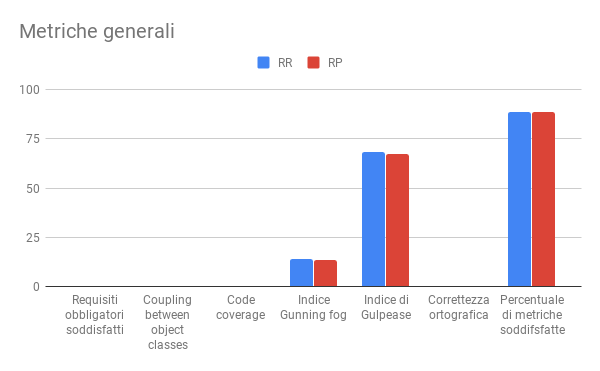
\includegraphics[width=0.99\linewidth]{res/images/metriche_generali.png}
	\caption{Diagramma di confronto - metriche generali}
\end{figure}

\begin{figure}[H]
	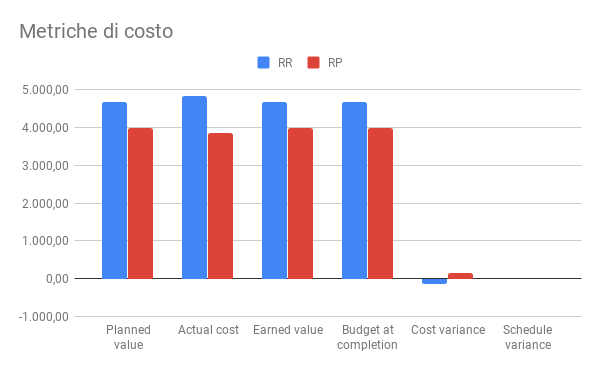
\includegraphics[width=0.99\linewidth]{res/images/metriche_costo.png}
	\caption{Diagramma di confronto - metriche di costo}
\end{figure}

\begin{figure}[H]
	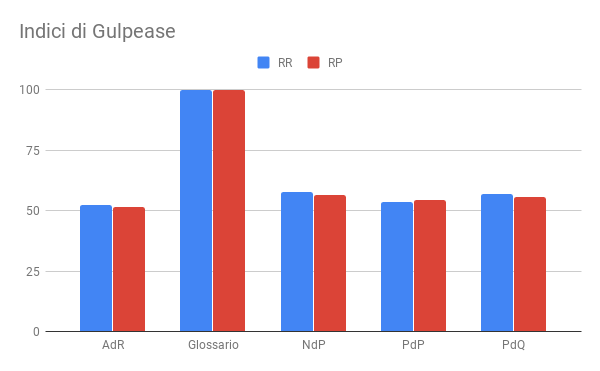
\includegraphics[width=0.99\linewidth]{res/images/indici_gulpease.png}
	\caption{Diagramma di confronto - indici di Gulpease}
\end{figure}

\begin{figure}[H]
	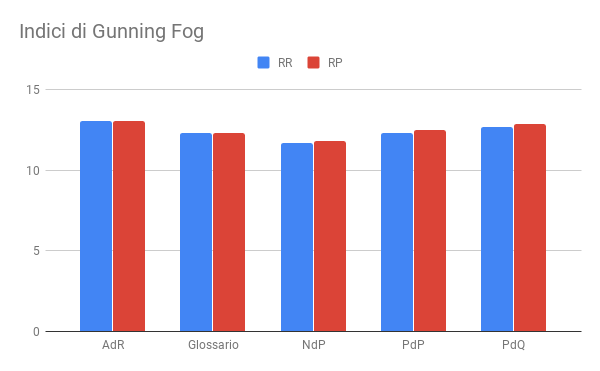
\includegraphics[width=0.99\linewidth]{res/images/indici_gunning_fog.png}
	\caption{Diagramma di confronto - indici di Gunning Fog}
\end{figure}